\chapter{Conclusion and Future Work}
\label{ch:conclusion}
\section{Conclusion}
\section{Future work}

\subsection{Sandbox Labs: a desktop client with local sandboxes}
\label{sec:desktop-client}
The pilot runs every student program on the college VM, which keeps the
runner simple but rules out a real terminal per student: sixty live Linux
shells on one VM would cost far more than today's short runs. A planned
\emph{Sandbox Labs} feature (Figure~\ref{fig:desktop-client}; full plan in
\texttt{thesis/plans/2026-10-30-desktop-client.md}) lets teachers set up their own
subjects and labs (an environment built from a checklist of tools rather than
a Dockerfile, assignments whose tests are checked against a reference
solution, and a library of labs teachers share with each other), each opened in a whole Linux instance per subject on the student's own
machine, with sudo, internet access for installing any tech stack (limited to
package registries in assessed labs), services and ports, a terminal, a file
tree, terminal editors such as vim, and our editor. Because a student is root
inside the instance, file, process and network capture runs in a sidecar
container they cannot stop, while key timing is captured in the app itself.
The client is an Electron app whose installer also sets up its own container
engine (rootless Podman in a small WSL2 distribution on Windows or a
lightweight VM on macOS), so students need no Docker installation; the
student's files are snapshotted to the server so work follows them to another
machine, including from a lab PC that cannot run the sandbox to one that can;
cloud instances exist only for teachers to preview a lab. Electron uses the same Chromium engine as the web editor, so
keystroke timestamps mean the same thing in both, which matters when a
baseline learned in the browser is compared with work done in the app. The
recorder is shared code, so the detector and review need no change for editor
work. The terminal becomes a new logged surface: key timing tagged by where it
was typed (editor, shell prompt or a terminal editor), commands, and files
changed outside the editor, shown like pastes. Because a student controls
their own machine, the client cannot be made tamper-proof; instead batches are
signed and hash-chained, submissions are graded on the server, and at
submission the server checks every file against the typing evidence behind it.

\begin{figure}[ht]
  \centering
  \resizebox{0.9\linewidth}{!}{\tikzfig{desktop-client}}
  \caption{Planned Sandbox Labs client: code runs in a local container (or a
  a cloud instance for teacher previews), while events, workspace snapshots and submissions go
  to the college server, where the detector and review are unchanged.}
  \label{fig:desktop-client}
\end{figure}

The teacher side of Sandbox Labs is built (Figure~\ref{fig:sandbox-teacher}).
Teachers create subjects without approval and give each an environment chosen
from a base and a checklist of tools; the server renders it to a Dockerfile
that a build service outside the college VM turns into an image. A lab is a
list of assignments, each with a statement, starter files, a run command, tests
(input/output pairs or a test command, some hidden) and a private reference
solution. Before publishing, a Check step runs the tests in the lab's real
environment: the reference solution must pass and the starter should fail.
Labs can be shared to a library as snapshots that colleagues copy into their
own subjects. A teacher can try any lab as a student in a short-lived cloud
instance with a terminal; these previews are capped (three seats, one per
teacher, an idle stop and an hour at most, never the open internet) so that
the VM cost the design moved to students' machines does not come back. Only a
separate service holds the Docker socket, and previews never create study
sessions.

\begin{figure}[ht]
  \centering
  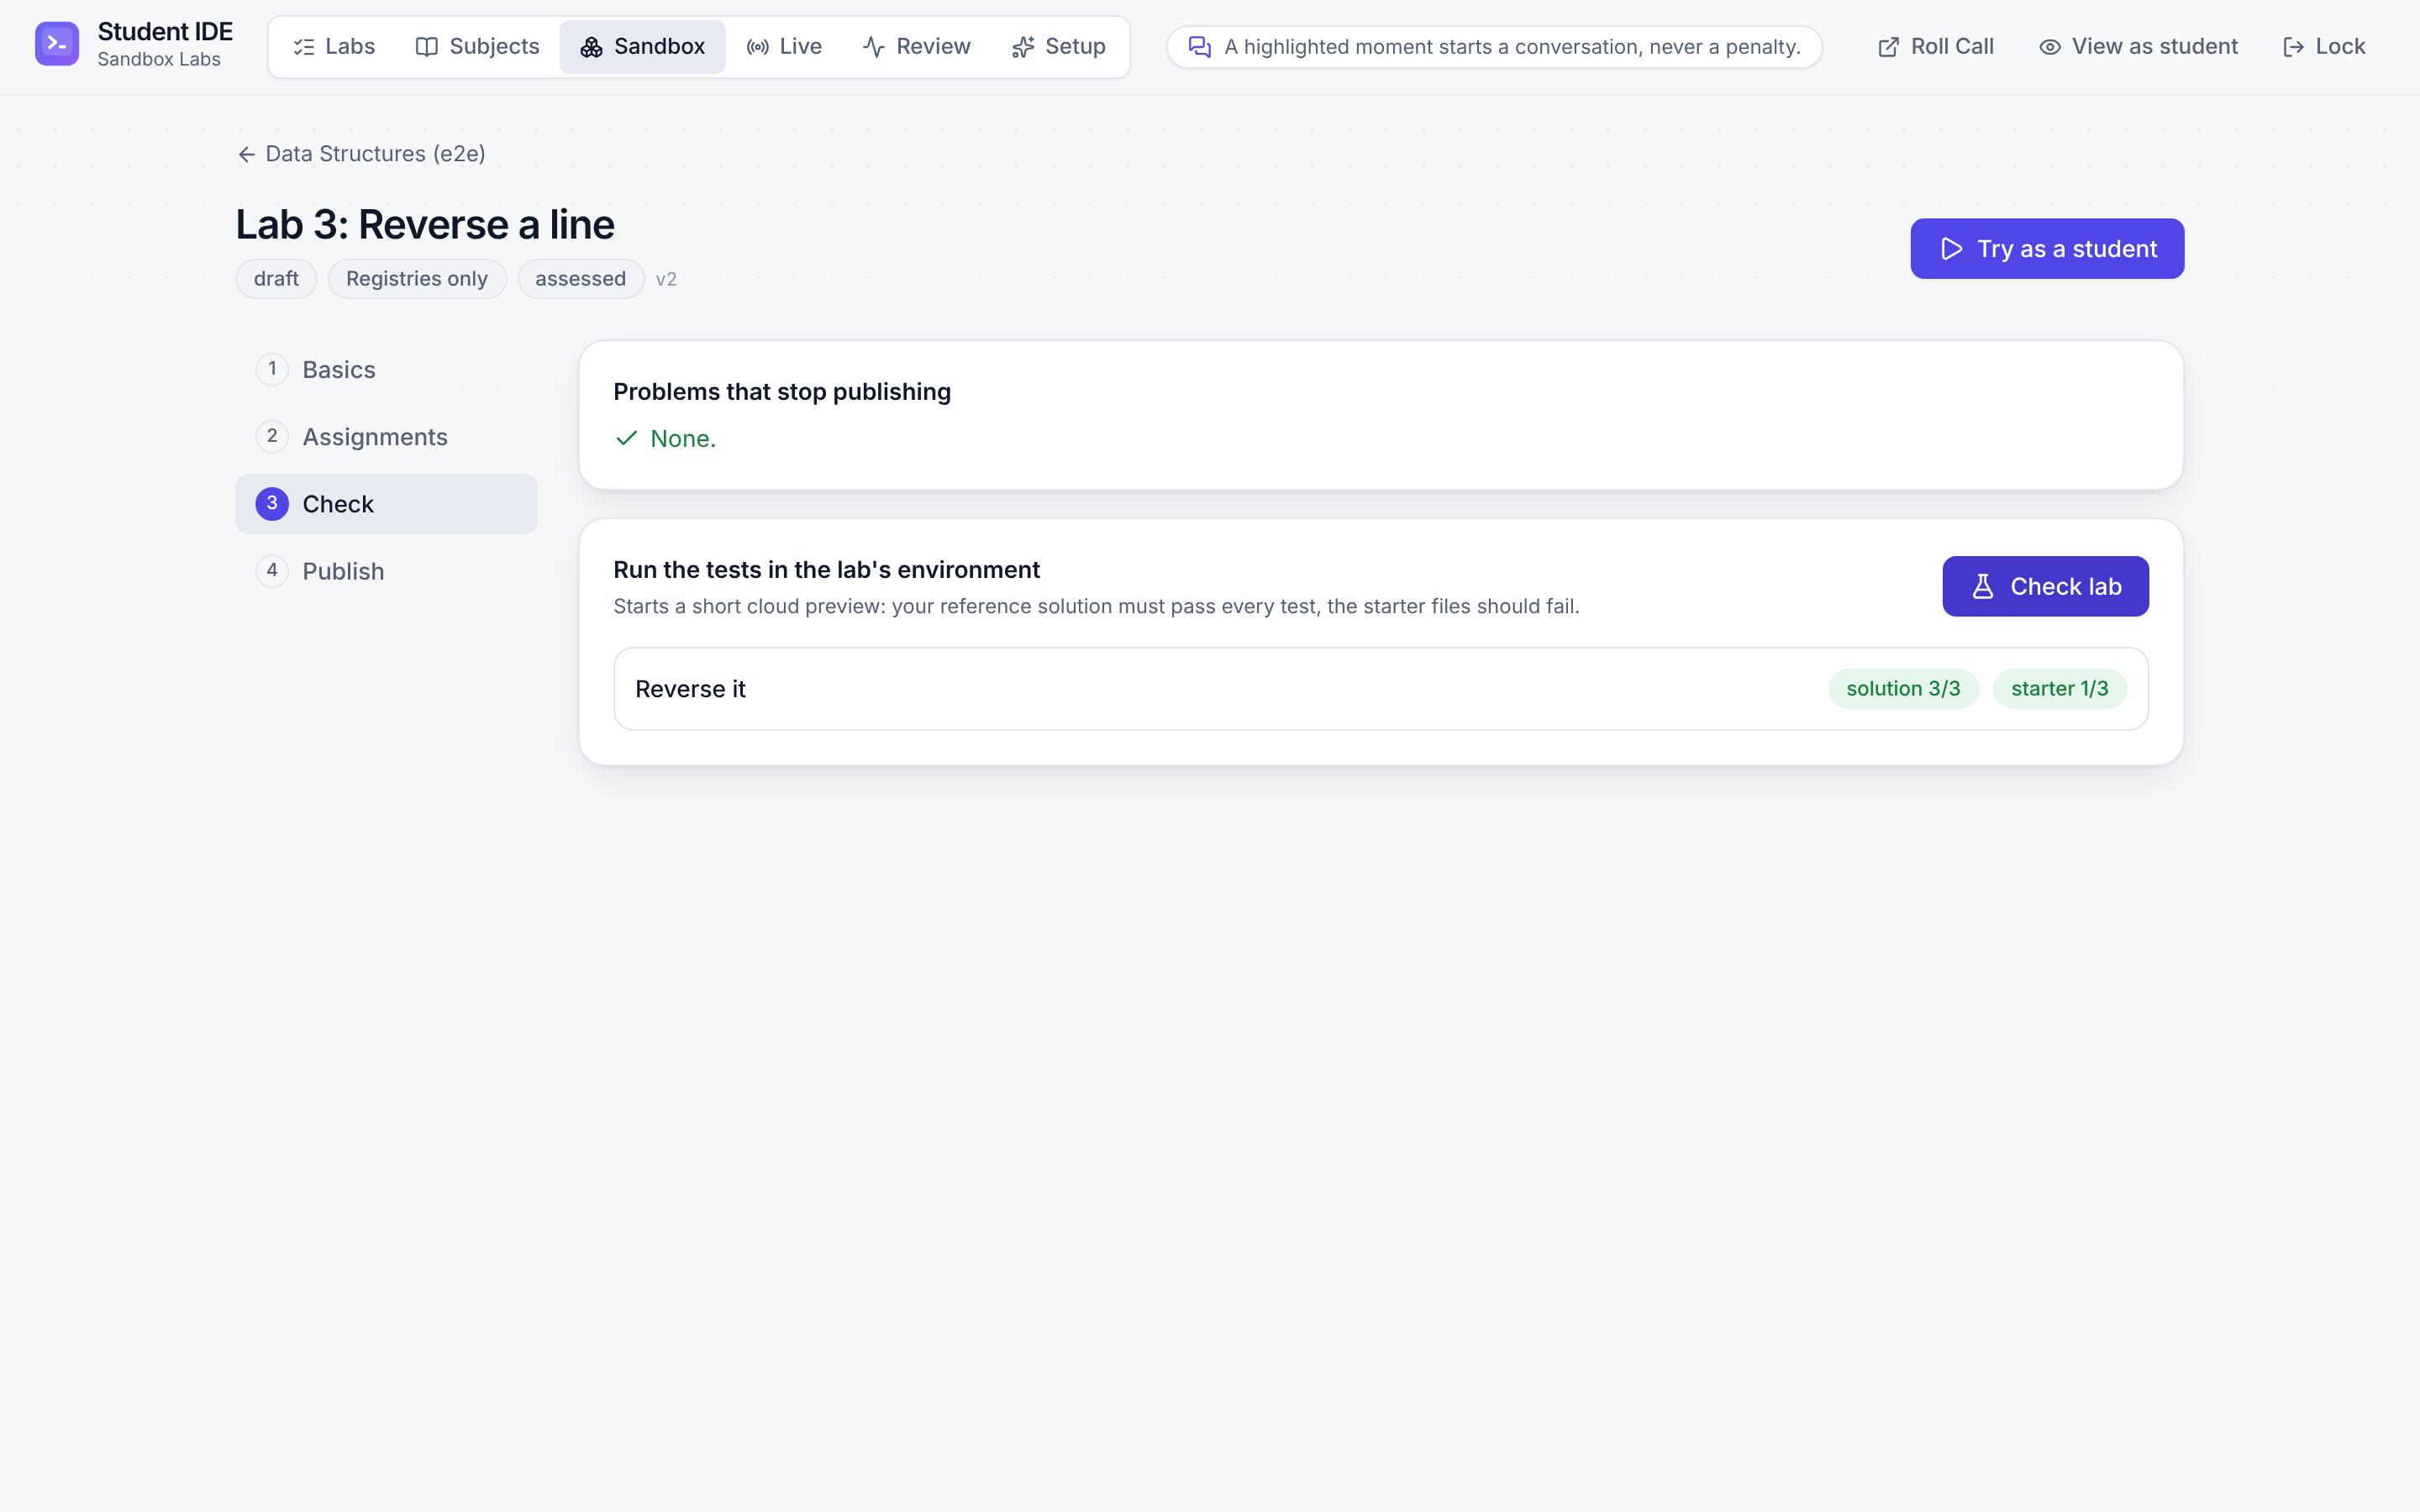
\includegraphics[width=0.49\linewidth]{sandbox/sandbox-light-05-check}\hfill
  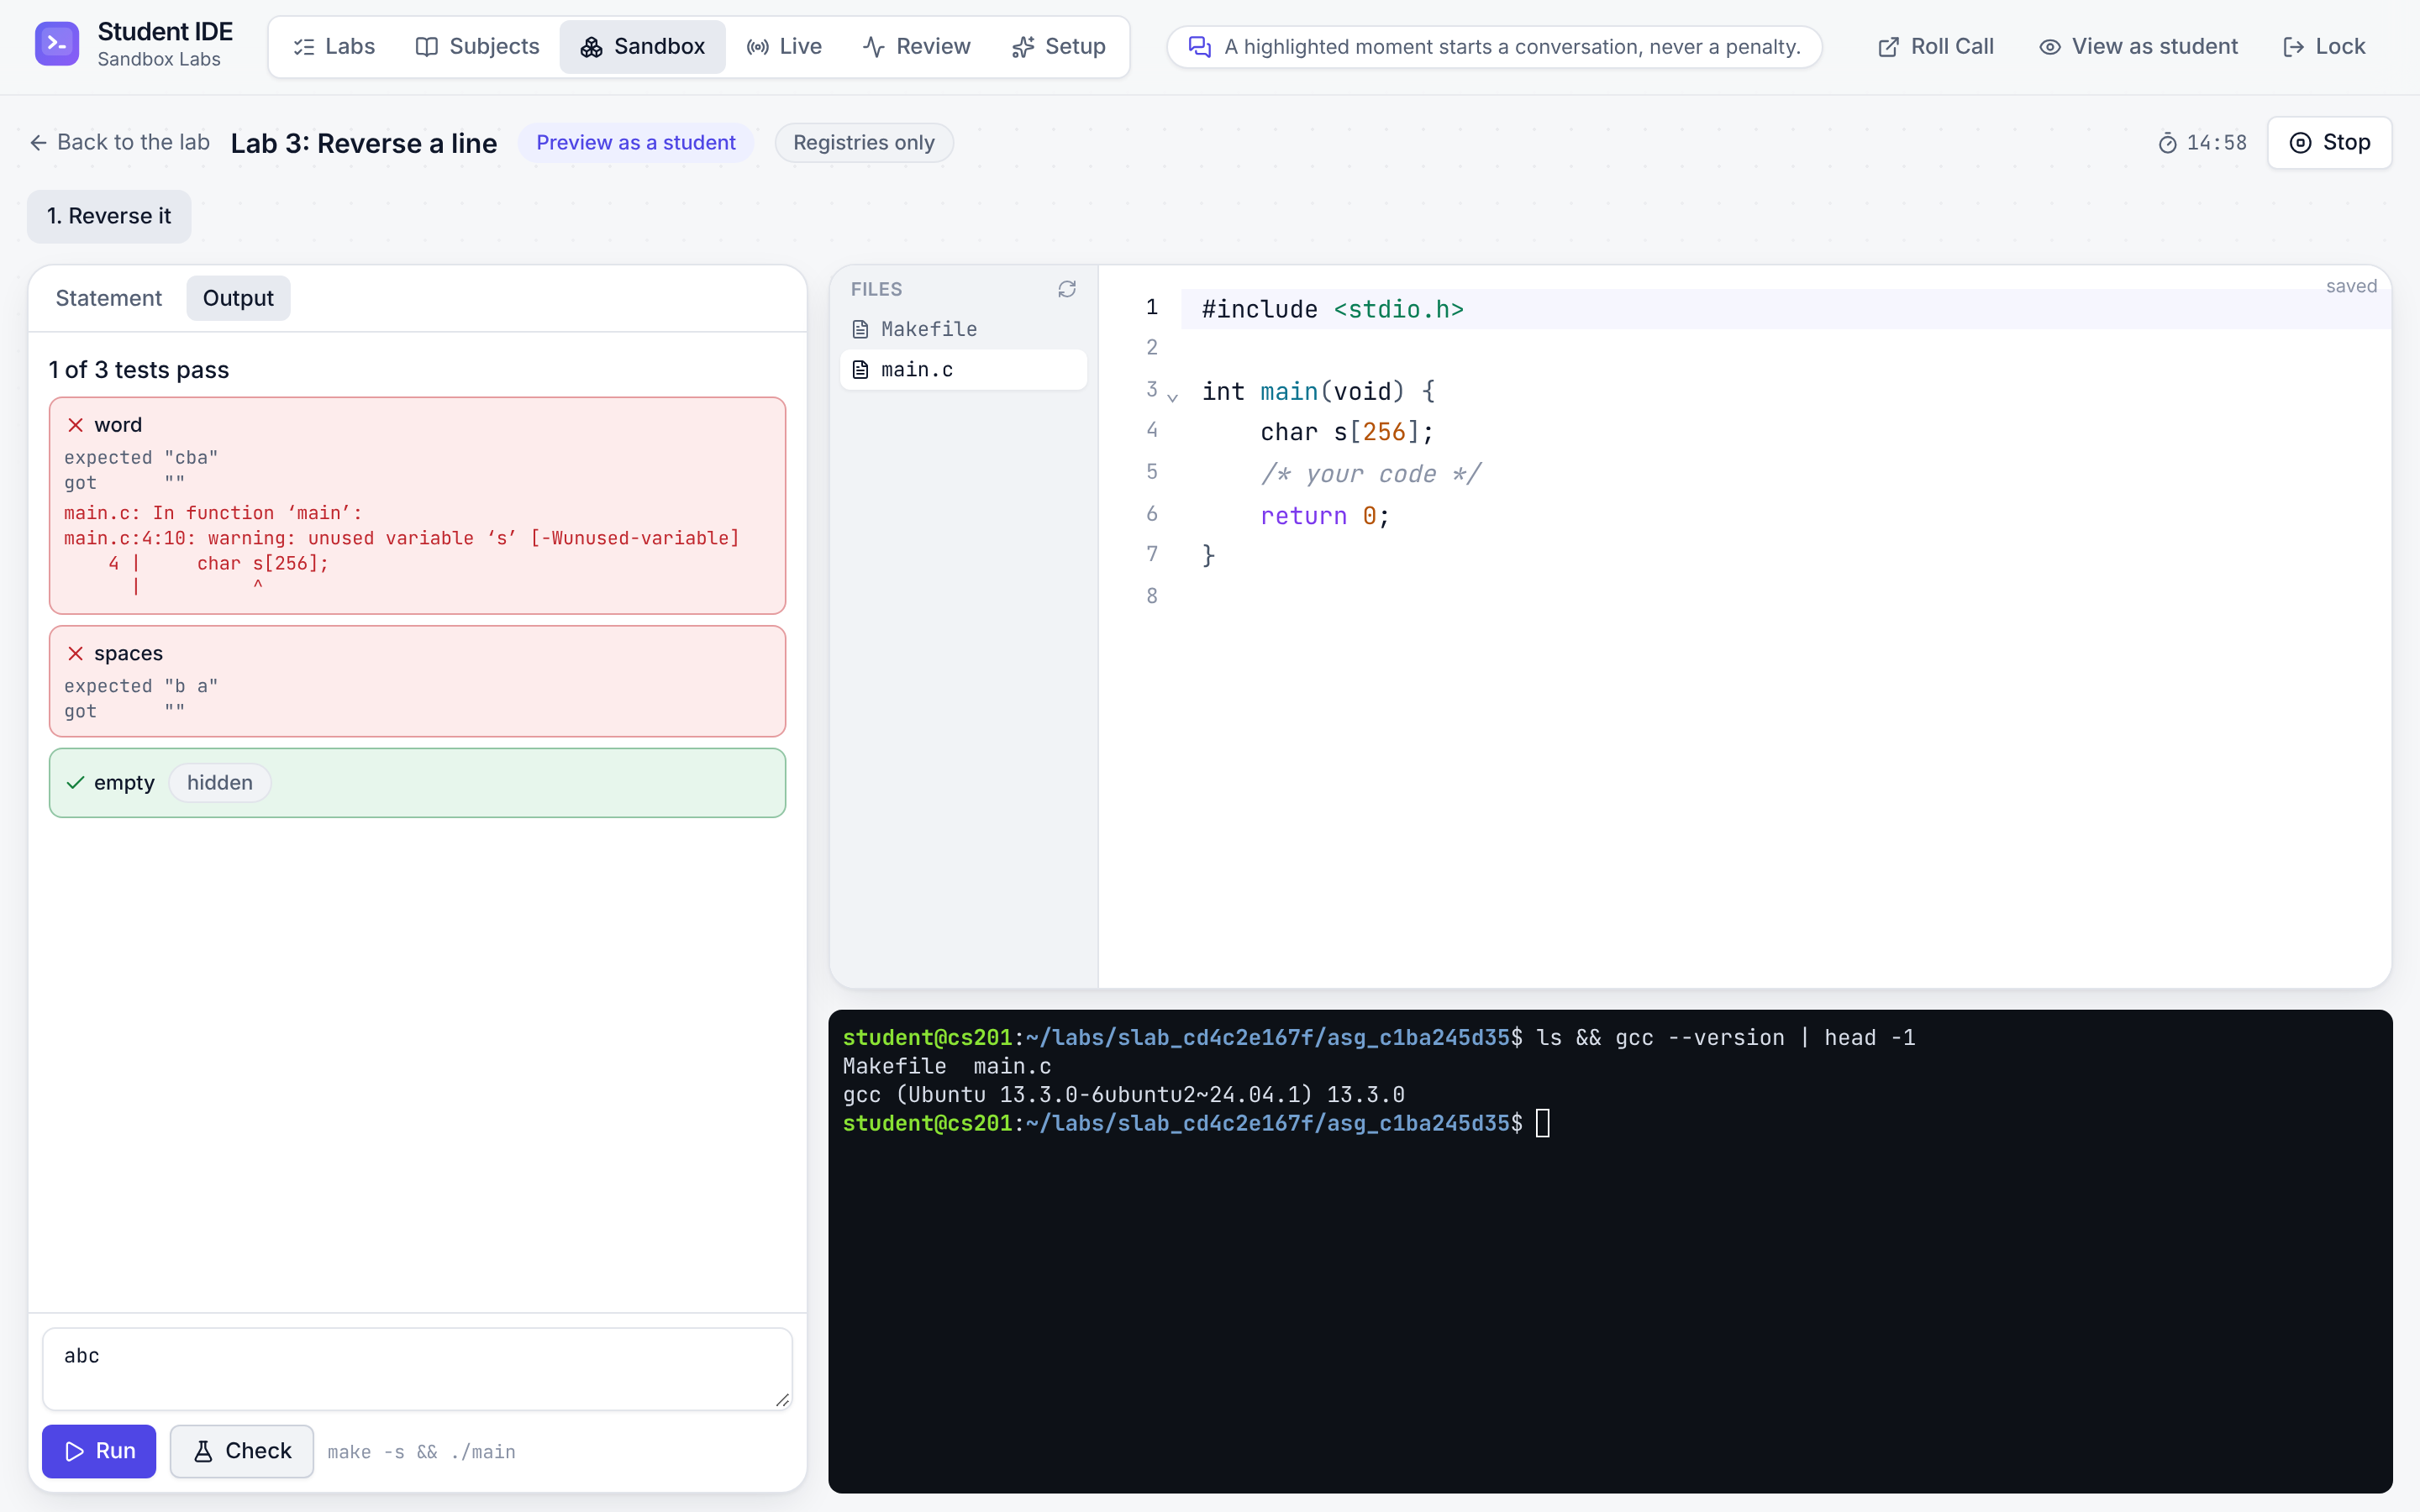
\includegraphics[width=0.49\linewidth]{sandbox/sandbox-light-06-try-as-student}
  \caption{Sandbox Labs, teacher side: the lab wizard's Check step (reference
  solution 3/3, starter 1/3) and ``Try as a student'' in a capped cloud
  preview with editor, terminal and the full test results.}
  \label{fig:sandbox-teacher}
\end{figure}
